\section{Systementwurf}

\subsection{Modellierung der Datenbank}

Um die Daten zu modellieren ist es sinnvoll, sich diese im Kontext der Erhebung zu betrachten. In (\ref{eq:datenstruktur}) ist dieser Prozess vereinfacht dargestellt.

\begin{equation}
    \mbox{Boje} \to (\mbox{misst}_{\mbox{zu Zeitpunkt}}) \to \mbox{Messprofile} \to ( \mbox{enhält} ) \to \mbox{Aufzeichnungen} \label{eq:datenstruktur}
\end{equation}

Dabei ist erkennbar, dass dieses Modell eine Verkettung von Entitäten und Ereignissen darstellt. Eine Boje misst über ihre Lebensdauer eine Anzahl von Messzyklen. Jeder dieser Messzyklen besteht aus einer gewissen Anzahl von Messwerten.

Um das Modell weiter fortzuführen, wurde diese Ereigniskette in ein Entitätsschema überführt. In Abbildung \ref{fig:ERM} ist eine mögliche Modellierung des Prozesses zu sehen. 

\begin{figure}[h!]
    \centering
    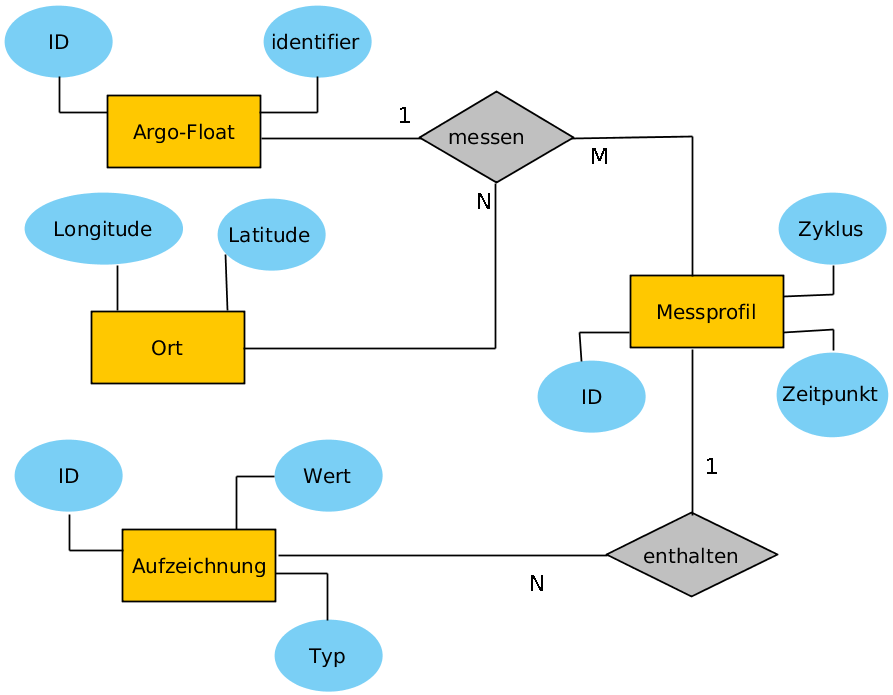
\includegraphics[width=0.6\textwidth,clip=true,trim=0pt 0pt 0pt 0pt]{pix/erm.png}
    \caption{Beschreibung der Entitäten der Datenaggregation}
    \label{fig:ERM}
\end{figure}



    
   
\subsection{Architektur}
    
        % TODO Darstellung der geplanten Systemarchitektur


Die Applikation besteht aus zwei Grundkomponenten. Ein Teil ist für die Beschaffung und Aufbereitung der Daten zuständig, während der zweite Teil für die Darstellung der Daten zuständig ist. 

% BEGIN OOP ARCHITEKTUR   AGGREGATION
\subsubsection{Entwurf der Datenaggregation}
\begin{figure}[h!]
\centering
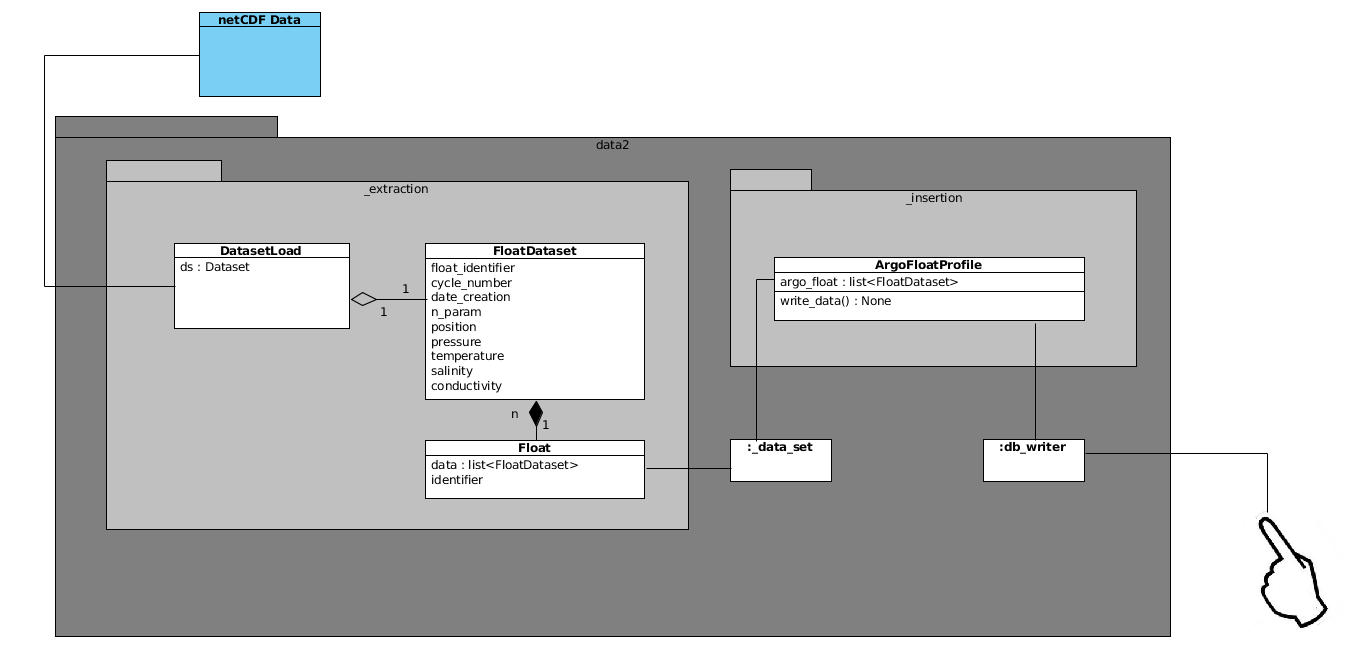
\includegraphics[width=\textwidth]{pix/grobentwurf_dataaggregation.png}
% grobentwurf_dataaggregation.png: 1436x727 px, 96dpi, 37.99x19.23 cm, bb=
\caption{Entwurf der Architektur der Aggregation der Daten}
\label{fig:grobetwurf_architektur_datenaggregation}
\end{figure}

Die Datenaggregation erfüllt zwei Funktionen. Zum einen muss sichergestellt sein, dass die Daten aus den vom Argo Programm bereitgestellten Strukturen gelesen und in ein logisches Format überführt werden. Des weiteren müssen diese Daten in die datenbank der Applikation überführt werden.

Auch in diesem Modell ist die Ereigniskette aus (\ref{eq:datenstruktur}) Abzubilden. Jede Messstation wird über ein Objekt abgebildet. Die hier gespeicherten Daten sind für eine Messstation eindeutig. Jeder Messzyklus der Boje wird über ein weiteres, zur Messstation gehöriges Objekt abgebildet. Dieses ist innerhalb des Kontextes eindeutig und trägt die Informationen zur jeweiligen Messung.

Für die Persistierung  werden objektorientierte Strukturen für den ORM verwendet. Diese Strukturen teilt sich das Modul mit der Webapplikation. Die Behandlung der Daten sowie eine Steuerung des Prozesses sind als weitere Schnittstellen zu definieren. 

Die Aggregation der Daten wird über zwei Teilbereiche abgebildet. Zum einen müssen die benötigten Parameter aus den Dateien ausgelesen und modelliert werden. 

Als zweite Ebene der Aggregation ist der Prozess des Schreibens in eine Datenbank zu sehen. Diese verwendet die zuvor ermittelten modellierten Messprofile und schreibt sie Anhand der dort enthaltenen Daten in eine Datenbank.


Es ist an dieser Stelle zu erkennen, dass zwei Stellen existieren, die die intrinsischen Eigenschaften des Modules an dieser Stelle beeinflussen. Hier sollten Schnittstellen geschaffen werden, die eine richtige Handhabung festsetzen

\paragraph{Schnittstellen}

\begin{enumerate}

\item \textbf{Daten}  
    \begin{enumerate}
        \item Die Datenstruktur ist normiert. Es ist sicherzustellen, dass die bekannte Daten- bzw Ordnerstruktur abgearbeitet wird. Mit Änderungen in dieser Struktur muss nicht gerechnet werden.
        \item Es muss sicher gestellt werden, dass geöffnete Dateien wieder geschlossen werden
    \end{enumerate}

\item \textbf{Steuerung} 
    \begin{enumerate}
        \item Daten separiert in die Datenbank zu schreiben, könnte zu Inkonsistenzen führen und soll vermieden werden.
        \item Der Prozess sollte als Sequenz modelliert werden.
        \item Es muss sicher gestellt werden, dass die Daten schrittweise in die Datenbank überführt werden. Würden zu Beginn alle Dateien geöffnet und gemeinsam im flüchtigen Speicher vorgehalten· könnte es zu Problemen führen.
    \end{enumerate}

\end{enumerate}

% END
        
% BEGIN OOP ARCHITEKTUR   WEBAPPLIKATION

\subsubsection{Entwurf der Webapplikation}

Die Webapplikation besteht aus zwei Teilkomponenten. Die erste Komponente ist für die Darstellung der Webseite zuständig. Durch diese wird HTMl Und Javascript ausgeliefert, welches im Webbrowser der Benutzenden angezeigt werden kann.

Die zweite Teilkomponente ist dafür zuständig, die für die Anzeige benötigten Daten bereitzustellen. Die hier bereitgestellte API ist Zustandslos und dient als Schnittstelle zur Auswahl und Anzeige von Datensätzen aus dem Backend. 

\subsubsection{Ausarbeitung der Webrouten}

\begin{python}
GET     /

GET     /argo_float/[identifier]
GET     /argo_float/[identifier]/[data]
GET     /last_seen
GET     /last_seen/[force_reload]
\end{python}


Die darstellende Schicht verfügt nur über eine einzige Webseite. Über das Root-Element der Webapplikation wird die Karte mit den Messstationen ausgeliefert. Interaktionen und Veränderte Daten werden nach dem \textit{singlepage-Prinzip} über diese Seite verfügbar gemacht.

Die API der Applikation soll zwei Funktionen erfüllen können. Für die Positionsbestimmung auf der Karte wird eine Geojson benötigt. Unter der Route \texttt{/last\_seen} finden sich die letzten Positionen der Mesststationen zusammen mit den Daten die beim Mouseover angezeigt werden sollen. Das hier zurückgegebene Geojson wird über einen Cache vorgehalten. Um diesen Cache neu zu generieren ist es möglich der Route die Variable \texttt{[force\_reload]} zu übergeben. Um versehendliche oder böswillige Verwendungen dieser Route zu verhindern, handelt es sich bei der Variable um ein Geheimnis. Nur wenn dieses richtig angegeben wird, werden die Daten neu erstellt.

Über die Route \texttt{argo\_float/[identifier]} wird ein Datensatz der über \texttt{identifier} ausgewählten Messstation zurückgegeben. Um nur einen spezifischen Messdatensatz zu erhalten, kann dieser über die Variable \texttt{data} ausgewählt werden. \\


Um die beiden Teilbereiche logisch zu trennen und modular vorhalten zu können, werden diese über blueprints abgebildet.


% END

% BEGIN DESIGN DARSTELLUNG
\subsubsection{Aussehen der Webapplikation}
%
%
% - Darstellung der Daten -- ...

Das Aussehen der Applikation soll dem Muster von gängigen Webapplikationen entsprechen. In Abbildung \ref{fig:entwurf_webseite} ist ein erster Grobentwurf der Applikation zu sehen.

Zentrales element der Applikation ist die Darstellung einer Karte. Über diese sollen die letzten Positionen der Karte ersichtlich sein.


Klickt man eine Messstation an, so wird auf der linken Seite ein weiteres Element ind ie Seite eingefügt. Dieses dient zur Darstellung der Messwerte des jeweiligen ArgoFloats.



\begin{figure}[h!]
    \centering
    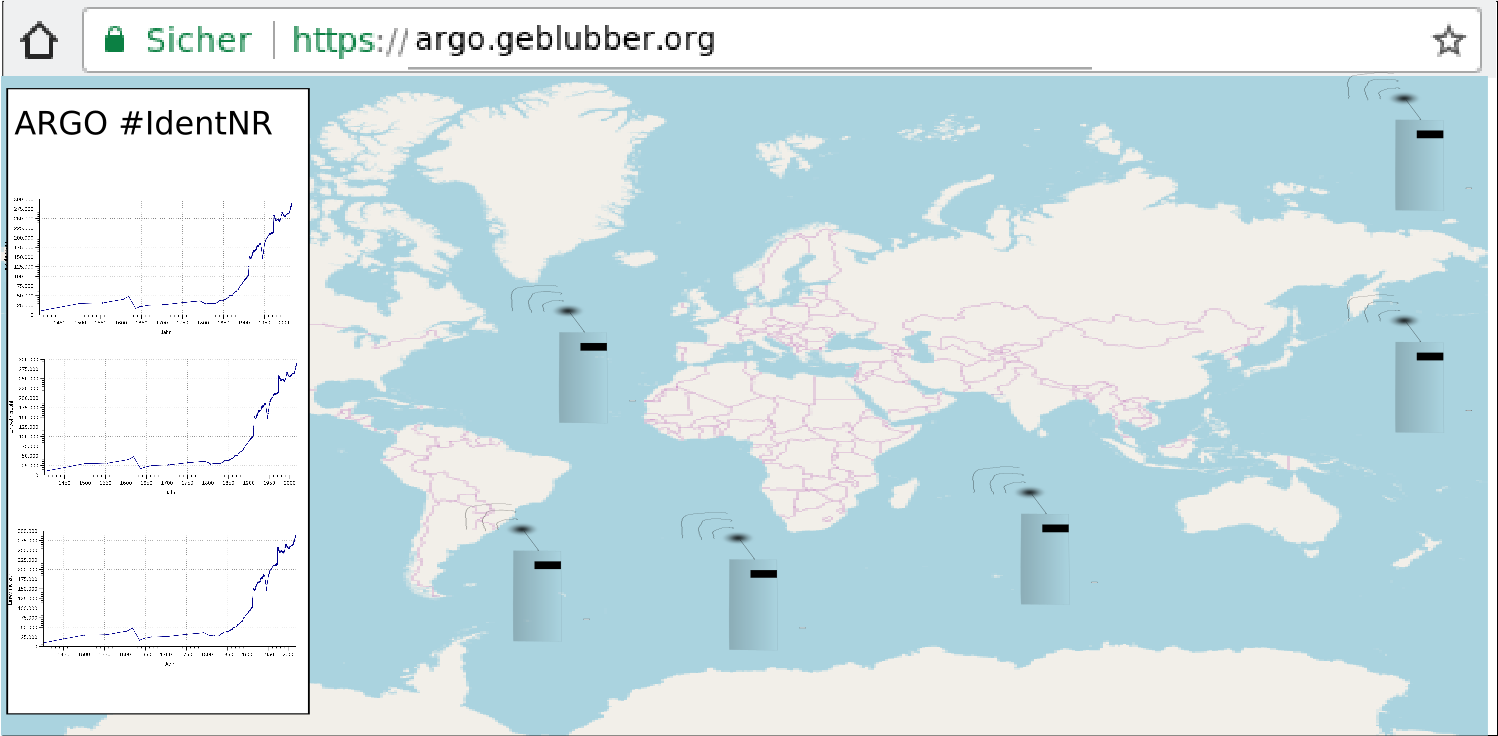
\includegraphics[width=\textwidth]{pix/EntwurfWebseite.png}
    % Entwurf_Webseite.svg.png: 1498x736 px, 96dpi, 39.63x19.47 cm, bb=0 0 1123 552
    \caption{Grafischer Grobentwurf der Webapplikation}
    \label{fig:entwurf_webseite}
\end{figure}

% END
